\section{Testing the Software}

\subsection{Rendering (\ref{req_rendering})}

\subsubsection{High Quality Rendering (1.1, 1.2, 1.3 and 1.4)}

These requirements revolve around correctly and accurately rendering fractals, which the images below demonstrate. The left image shows the Mandelbrot set, with the right image (a zoomed-in portion of the former) showing that there are no artefacts in the render. Both images are pleasantly coloured and the details of the fractal are clearly highlighted.

\FloatBarrier
\begin{figure*}[htp]
	\centering
	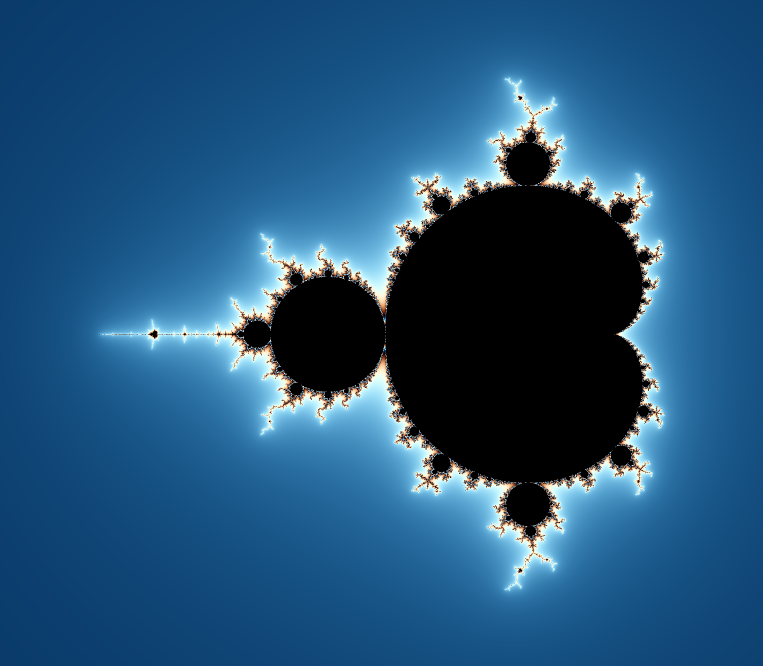
\includegraphics[width=.435\textwidth]{requirement1.1.png}
	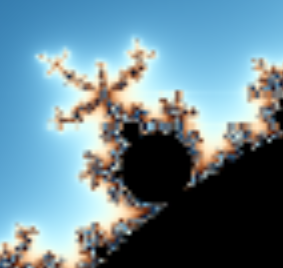
\includegraphics[width=.4\textwidth]{requirement1.1_2.png}
\end{figure*}
\FloatBarrier

\subsubsection{Anti-Aliasing (1.5)}

Anti-aliasing the render makes it appear much smoother and reduces pixelation in the image. The two images below show the difference between rendering the image with and without anti-aliasing (they are rendered at a low resolution to emphasise the differences). The image on the right is rendered with anti-aliasing, while the image on the left is not.

\FloatBarrier
\begin{figure*}[htp]
	\centering
	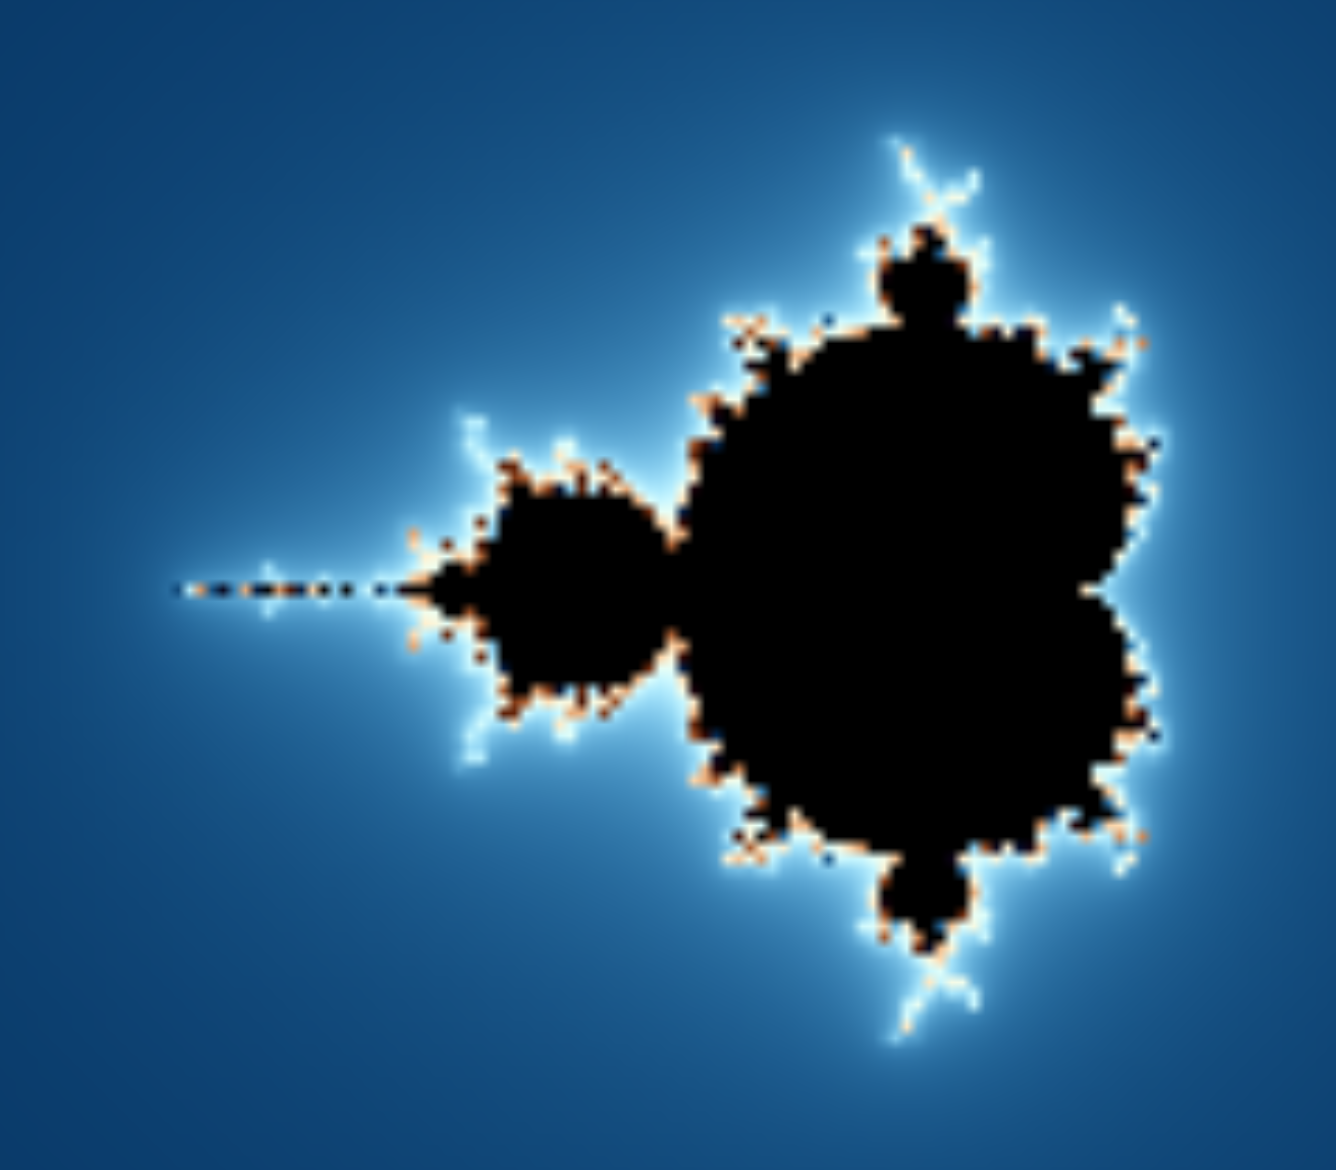
\includegraphics[width=.4175\textwidth]{requirement1.5.png}
	
\includegraphics[width=.4175\textwidth]{requirement1.5_2.png}
\end{figure*}
\FloatBarrier

\subsubsection{Image Resizing (1.6)}

The images below show the same portion of the Mandelbrot set, but rendered at different resolutions. The lower the resolution, the quicker the image is to render, but the worse it looks.

\FloatBarrier
\begin{figure*}[htp]
	\centering
	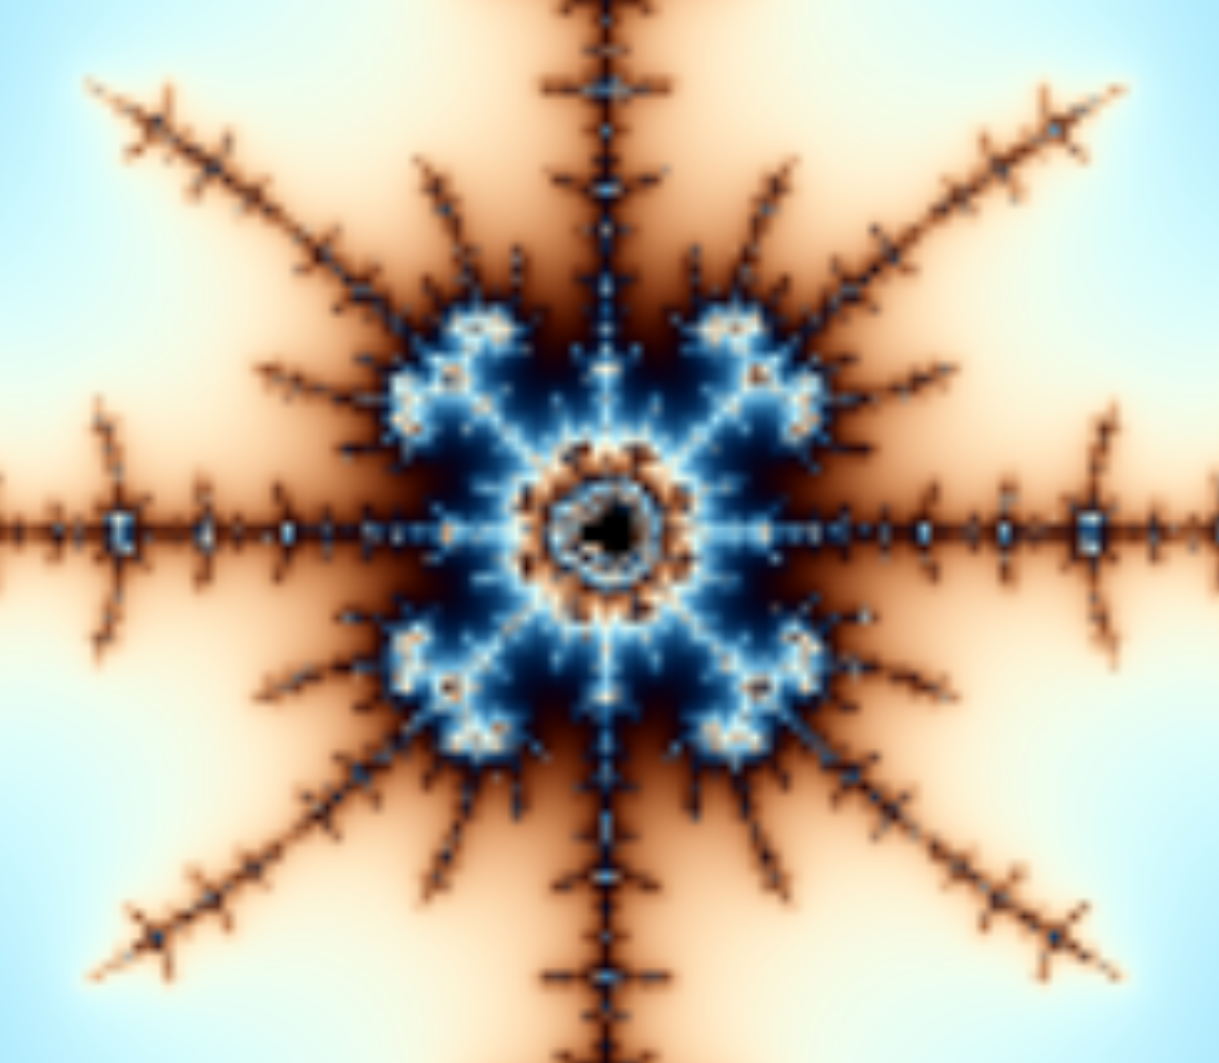
\includegraphics[width=.4175\textwidth]{requirement1.6.png}
	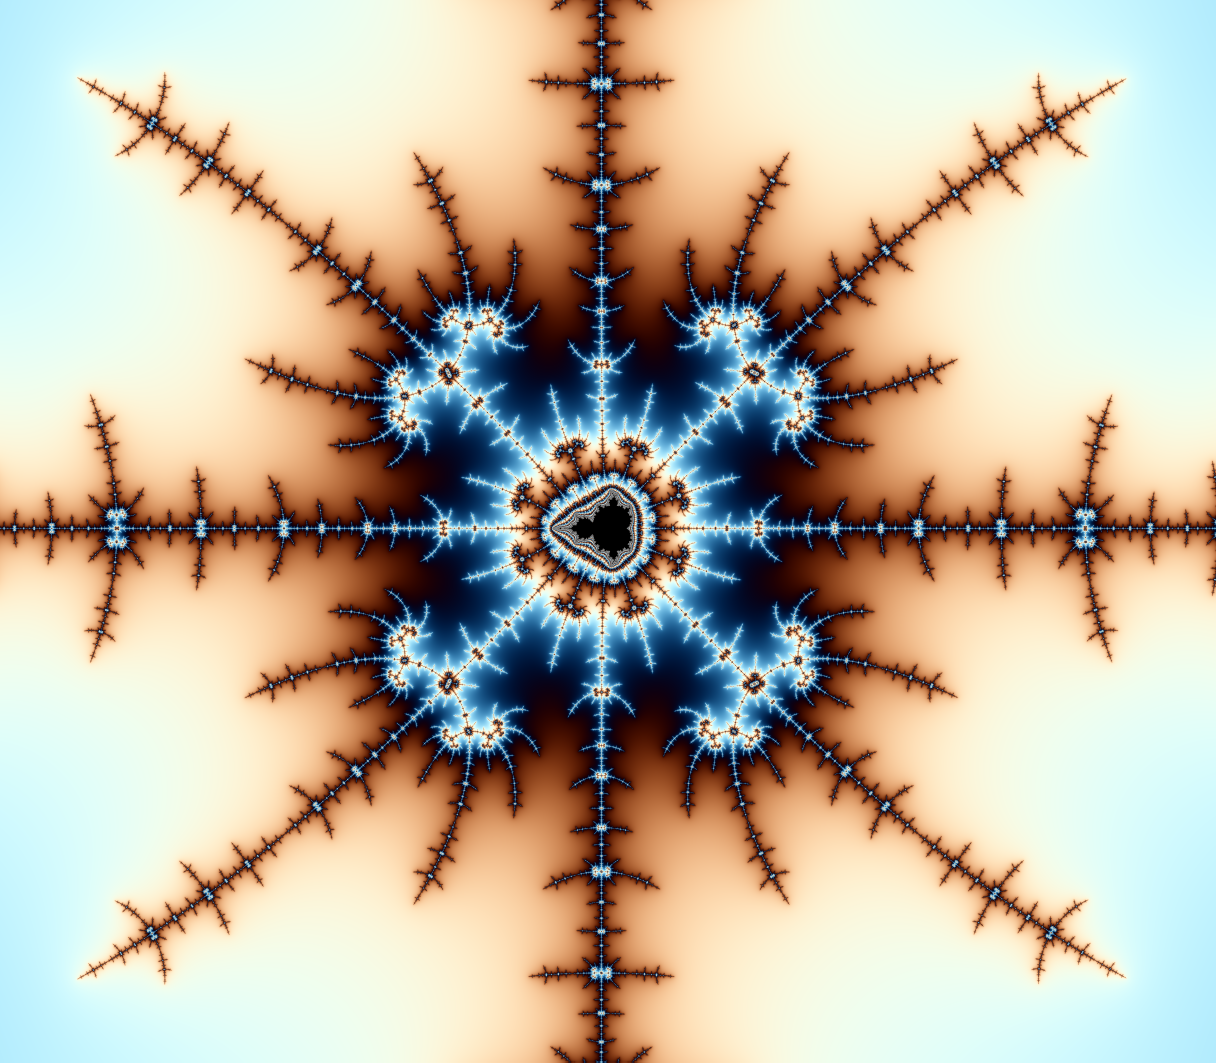
\includegraphics[width=.4175\textwidth]{requirement1.6_2.png}
\end{figure*}
\FloatBarrier

\subsubsection{Optimisations (1.7, 1.8)}

The only algorithmic optimisation that was practical to implement within the scope of this project was the outline detection method of accelerating the rendering of some regions of the fractal. The image below shows, in red, the render boxes whose perimeters were entirely contained within the Mandelbrot set and hence contain only points in the set.

\FloatBarrier
\begin{figure*}[htp]
	\centering
	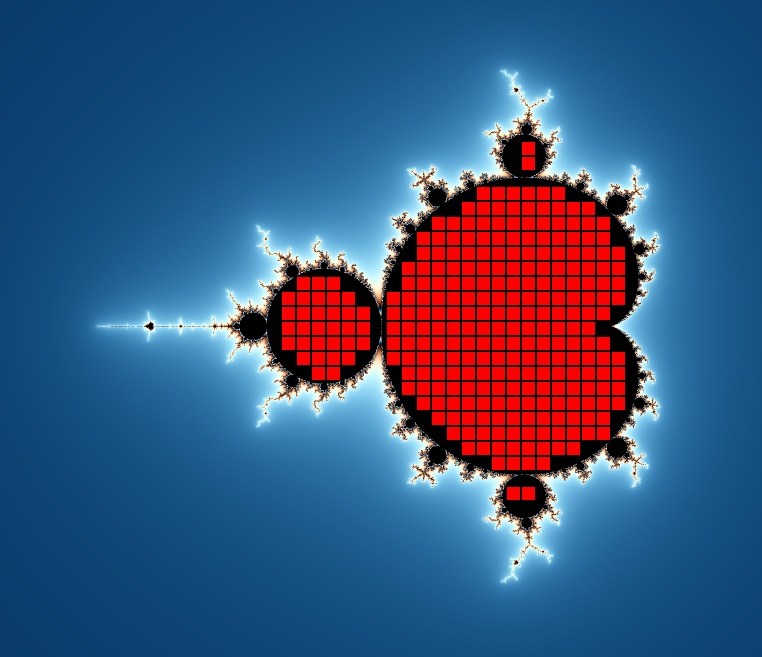
\includegraphics[width=.835\textwidth]{requirement1.8.png}
\end{figure*}
\FloatBarrier

\subsubsection{Infinite Zooming (1.9)}

When the user zooms in to a factor of around $1 \times 10 ^{14}$, the precision of a 64-bit floating point value leads to significant rendering artefacts. To circumvent this, the program has support for arbitrary-precision floating point types, which are implemented in software. These make the rendering process much slower, but allow for near-infinite zooming.

The image on the left shows the fractal rendered with 64-bit precision, while the image on the left shows the same point rendered with 128-bit precision.

\FloatBarrier
\begin{figure*}[htp]
	\centering
	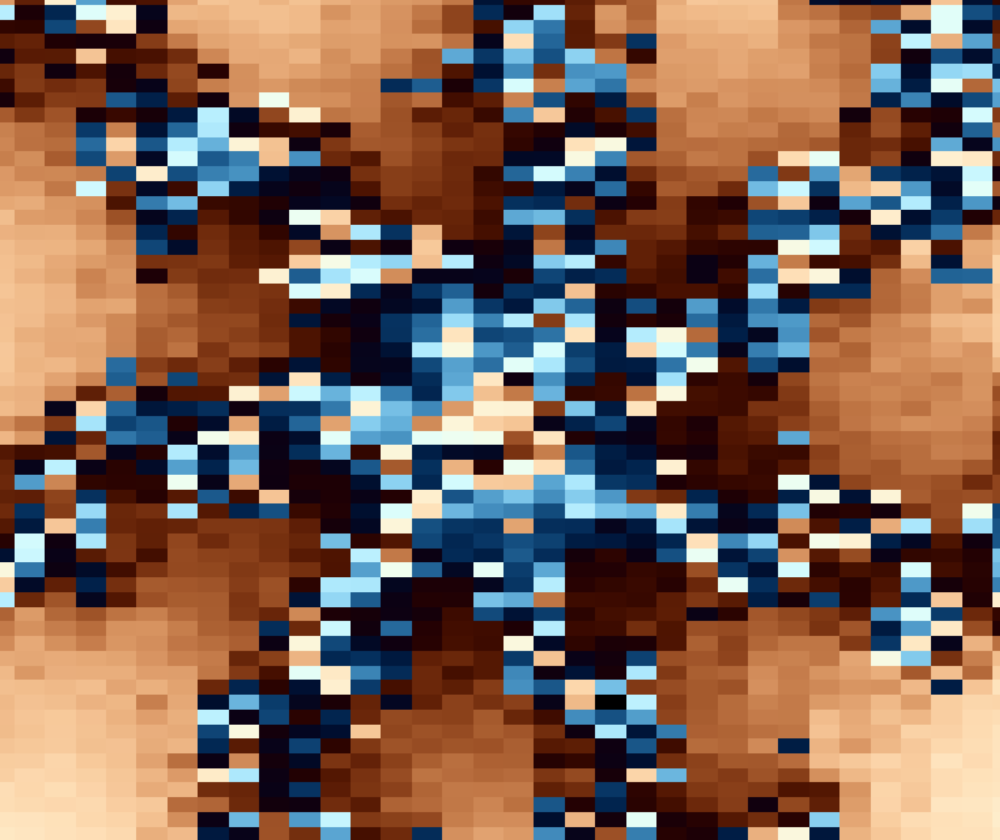
\includegraphics[width=.4175\textwidth]{requirement1.9.png}
	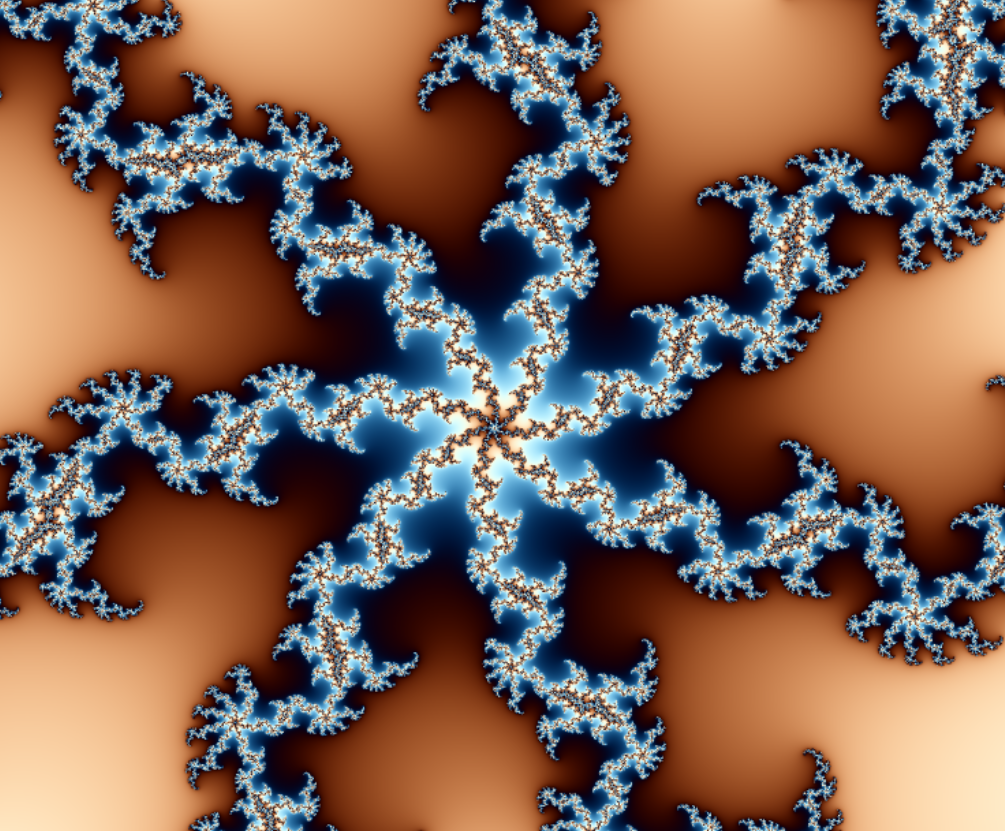
\includegraphics[width=.4175\textwidth]{requirement1.9_2.png}
\end{figure*}
\FloatBarrier


\subsection{Configuration (\ref{req_configuration})}

\subsubsection{Zoom Factor and Fractal Position (2.1)}

The zoom factor and fractal position can be adjusted in two main ways. The first way is to change the \codeword{settings.json} file directly, entering custom coordinates and dimensions for the fractal. The second, and much easier way, is implemented and tested in various sections of requirement 3 (``Interface and Movement'').

\subsubsection{Fractal Render Configurations (2.2, 2.3, 2.4, 2.5)}

In order for the program to be fully customisable, the number of threads, anti-aliasing factor, etc. must be configurable. The window responsible for providing these options is shown below.

Note that, while the bailout value cannot be changed directly from this menu (since it does not significantly change the appearance of the resulting image), it can be changed from within the \codeword{settings.json} file.

\FloatBarrier
\begin{figure*}[htp]
	\centering
	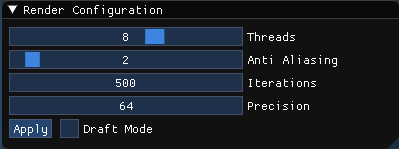
\includegraphics[width=.835\textwidth]{requirement2.2.png}
\end{figure*}
\FloatBarrier

\subsubsection{Image Resizing (2.6, 2.7)}

The ability to resize the image (both drawn size and rendered size) has been demonstrated in previous points (notably in 1.6)

\subsubsection{Colouring Algorithms (2.8)}

The colouring algorithm can be changed by selecting an option in a simple drop down menu. The images below show three different colouring methods applied to the same fractal. The middle two algorithms support custom colour palettes, which can be defined in the \codeword{settings.json} file and loaded from another drop down menu.

\FloatBarrier
\begin{figure*}[htp]
	\centering
	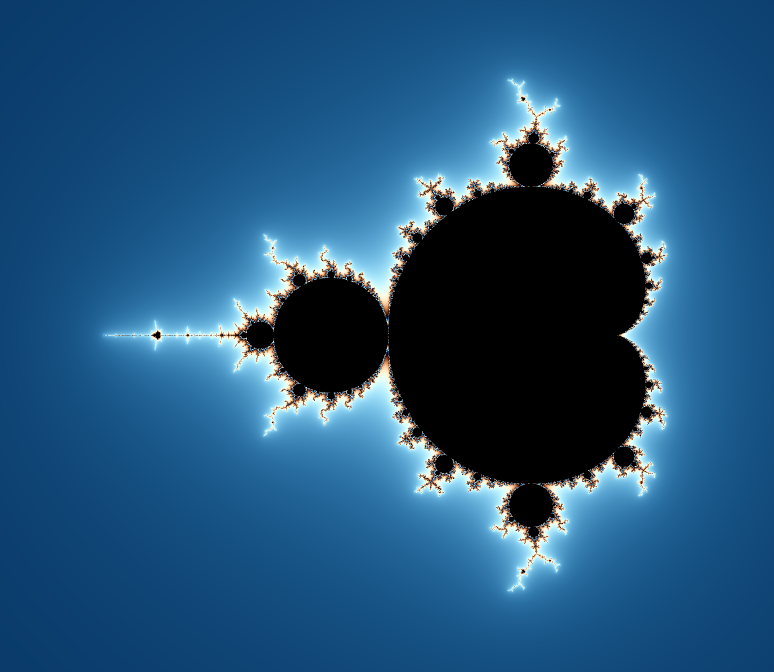
\includegraphics[width=.243\textwidth]{requirement2.8.png}
	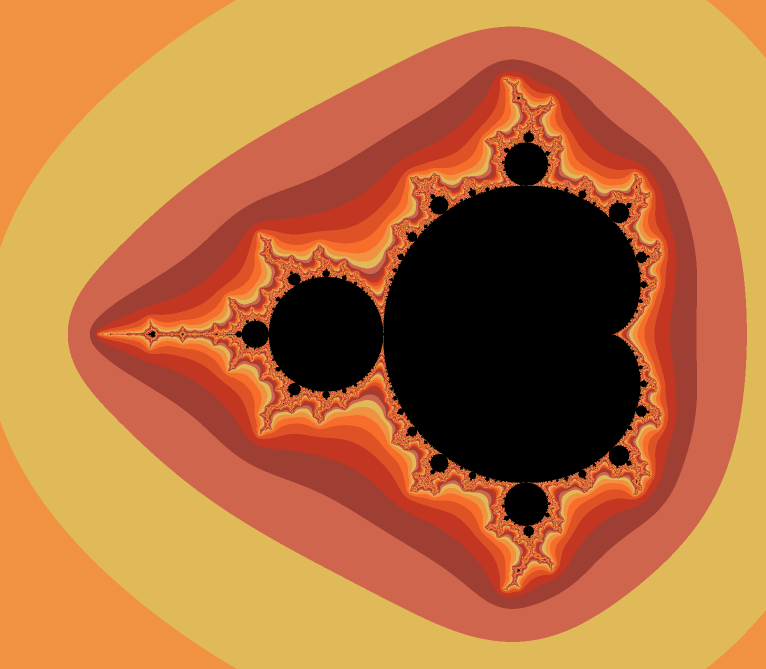
\includegraphics[width=.243\textwidth]{requirement2.8_2.png}
	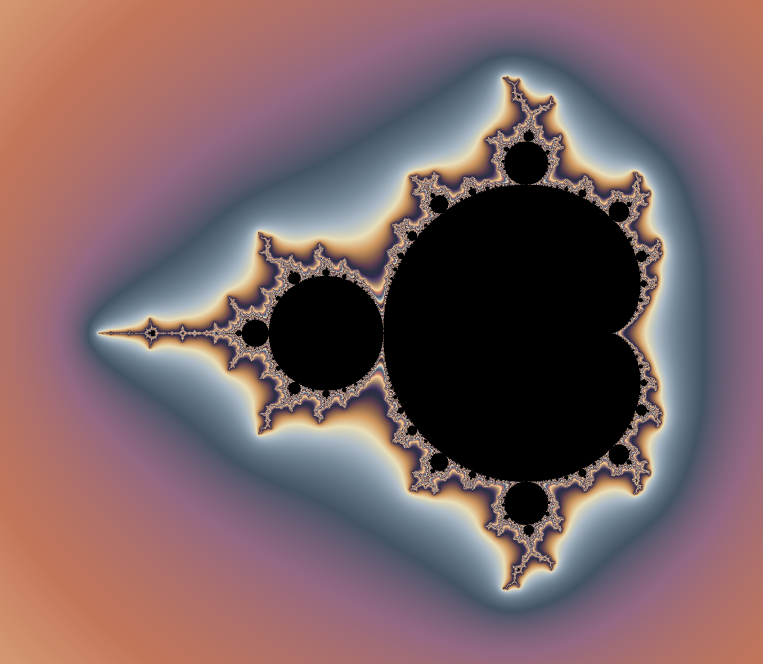
\includegraphics[width=.243\textwidth]{requirement2.8_3.png}
	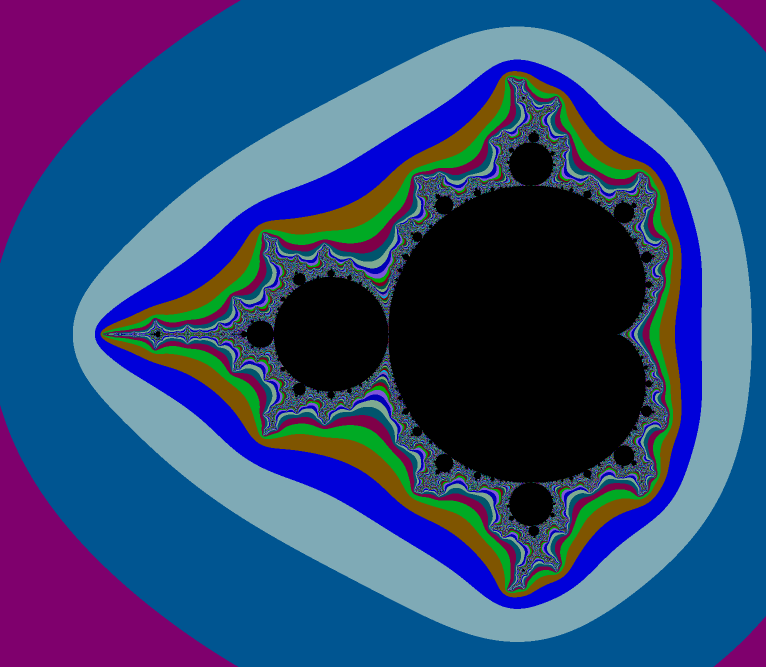
\includegraphics[width=.243\textwidth]{requirement2.8_4.png}
\end{figure*}
\FloatBarrier

\subsubsection{Default Settings (2.9)}

A single button in the \codeword{Fractal Settings} window enables the user to reset the fractal to its default configuration, which is defined by the \codeword{settings.json} file.

\subsection{Interface and Movement (\ref{req_interface})}

\subsection{Import and Export (\ref{req_import_export})}
	
\subsection{Installation (\ref{req_install})}

\subsection{Performance (\ref{req_performance})}
		
